\documentclass[conference]{IEEEtran}
\IEEEoverridecommandlockouts
% The preceding line is only needed to identify funding in the first footnote. If that is unneeded, please comment it out.
\usepackage{cite}
\usepackage{amsmath,amssymb,amsfonts}
\usepackage{algorithmic}
\usepackage{graphicx}
\usepackage{textcomp}
\usepackage{xcolor}
\usepackage{booktabs}
\usepackage{subcaption}
\usepackage{lipsum} 
\usepackage{dblfloatfix}

\def\BibTeX{{\rm B\kern-.05em{\sc i\kern-.025em b}\kern-.08em
    T\kern-.1667em\lower.7ex\hbox{E}\kern-.125emX}}

\makeatletter
\newcommand{\linebreakand}{%
    \end{@IEEEauthorhalign}
    \hfill\mbox{}\par
    \mbox{}\hfill\begin{@IEEEauthorhalign}
}
\makeatother

\begin{document}

% Title
\title{Development of Microcontroller-Based AI Robot Tour Guide Utilizing Custom Language Models
\thanks{Computational resources were provided by the WVU Research Computing Thorny Flat HPC cluster, partly funded by NSF OAC-1726534.}
}

% Authors 
\author{
    \IEEEauthorblockN{Ian S. Jackson}
    \IEEEauthorblockA{\textit{West Virginia University} \\
            Morgantown, United States \\
            isj0001@mix.wvu.edu}
    \and

    \IEEEauthorblockN{Aiden G. Ballard}
    \IEEEauthorblockA{\textit{West Virginia University} \\
            Morgantown, United States \\
            agb00033@mix.wvu.edu}

    \linebreakand

    \IEEEauthorblockN{Dr. Mohamed Hefeida}
    \IEEEauthorblockA{\textit{West Virginia University} \\
            Morgantown, United States \\
            mohamed.hefeida@mail.wvu.edu}

    \and

    \IEEEauthorblockN{Dr. Anurag Srivastava}
    \IEEEauthorblockA{\textit{West Virginia University} \\
            Morgantown, United States \\
            anurag.srivastava@mail.wvu.edu}
            
    \and

    \IEEEauthorblockN{Dr. Prashnna Gyawali}
    \IEEEauthorblockA{\textit{West Virginia University} \\
            Morgantown, United States \\
            prashnna.gyawali@mail.wvu.edu}
}

\maketitle
\thispagestyle{plain}
\pagestyle{plain}

%== ABSTRACT ==%
\begin{abstract}
    This paper presents the design and implementation of an AI-powered robotic tour guide system for the Lane Department of Computer Science and Electrical Engineering (LCSEE). 
    The system enables prospective students to engage in real-time, natural language conversations with a robot equipped with department-specific knowledge. 
    Two methodologies were explored: (1) a DirectLLM approach that fine-tunes a large language model on a custom dataset, and (2) a Classify-Retrieve-Generate (CRG) pipeline that modularizes classification, answer retrieval, and natural response generation. 
    A custom SQuAD-style dataset was developed using LCSEE data, supporting both pipelines. 
    The system was deployed on a Raspberry Pi 4 integrated with a MangDang Mini Pupper robot. 
    Evaluation results show that while DirectLLM excels in fluency, it suffers from retraining constraints and scalability issues. 
    In contrast, the CRG method provides modularity and easier maintenance, with strong performance on classification and retrieval but pending refinement in response generation. 
    Future work includes dataset expansion, CRG generator improvements, DirectLLM fine-tuning, and exploration of hybrid fusion models. 
    This research demonstrates the feasibility of deploying compact, domain-aware AI agents for real-time educational engagement.
\end{abstract}

%== KEYWORDS ==%
% \begin{IEEEkeywords}
%     TODO: keywords
% \end{IEEEkeywords}

%== Introduction ==%
\section{Introduction}
Advancements in artificial intelligence (AI) and natural language processing (NLP) have enabled new forms of human-computer interaction, particularly in the realm of educational engagement. 
Universities increasingly seek innovative ways to connect with prospective students, providing them with immersive experiences that showcase academic programs, research opportunities, and campus life. 
One such approach is the integration of AI-powered robotic tour guides that allow visitors to interact dynamically with departmental resources.

This research focuses on the development of an AI-driven robotic tour guide designed to enhance the experience of prospective students visiting the Lane Department of Computer Science and Electrical Engineering (LCSEE). 
The goal is to create an interactive medium where students can ask questions about the department, and the robot, powered by language models, generates informative responses in real-time. 
Unlike static presentations or pre-scripted responses, this approach enables natural, context-aware interactions, providing a more engaging and personalized tour experience.

To achieve this, two distinct methodologies were explored: 
(1) DirectLLM, which fine-tunes a large language model (LLM) specifically for LCSEE-related queries, and 
(2) a Classify-Retrieve-Generate (CRG) pipeline, which first classifies the user's question, retrieves relevant information, and then generates a response. 
A custom Q\&A dataset was curated using LCSEE-specific data, ensuring that the AI model delivers accurate and contextually relevant information.

The system was deployed on a Raspberry Pi 4, paired with a MangDang Mini Pupper \cite{b1} robot as the physical embodiment of the tour guide. 
The robot is equipped with a simple microphone and speaker interface, facilitating natural language communication with users. 
The choice of hardware necessitated the use of a lightweight AI model optimized for fast inference, ensuring real-time conversational interactions without significant latency.

This paper details the design, development, and deployment of the AI-powered robotic tour guide, evaluating the performance of both DirectLLM and the CRG-based approach. 
By comparing these methods, we aim to determine the most effective strategy for delivering responsive and informative AI-driven interactions in an embedded robotics context.

% System diagram
\begin{figure*}[t]
    \centering
    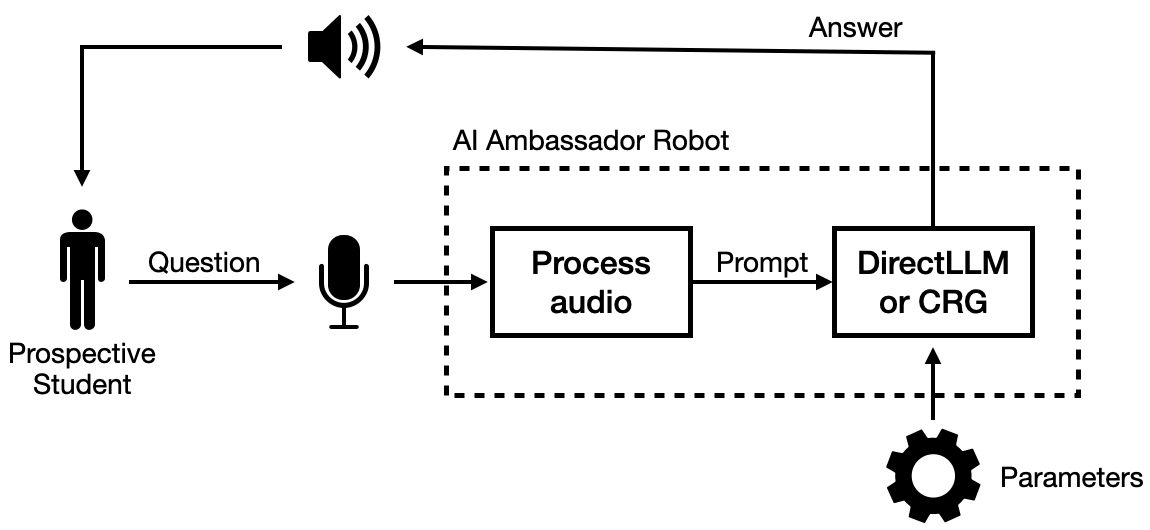
\includegraphics[width=0.70\linewidth]{assets/system_diagram.png}
    \caption{AI Robot System Diagram}
    \label{fig:system}
\end{figure*}

%== Related Work ==%
\section{Related Work}
\subsection{Fine-Tuning Large Language Models for Domain-Specific Tasks}
Fine-tuning pre-trained LLMs has become a standard approach to adapting general-purpose models for domain-specific applications. 
Studies show that fine-tuned LLMs outperform generic models in specialized domains, such as healthcare and legal services \cite{b2}, by leveraging tailored datasets. 
The DirectLLM approach in this work applies the same principle, fine-tuning a model specifically on Lane Department of CSEE (LCSEE) information. 
However, fine-tuning requires significant computational resources, which poses challenges for deployment on edge devices like microcontrollers and single-board computers \cite{b3}.

\subsection{Deploying AI Models on Resource-Constrained Devices}
Deploying AI models on low-power devices such as Raspberry Pi and microcontrollers presents unique challenges, primarily due to hardware limitations in memory and computation. 
Prior studies have explored optimization techniques such as quantization, pruning, and distillation to reduce model size while preserving accuracy \cite{b4}. 
Recent advancements in small language models (SLMs) offer promising alternatives for efficient, real-time inference \cite{b5}. 
This work integrates such optimizations to deploy a lightweight yet effective AI system on a Raspberry Pi 4.

%== System Overview ==%
\section{System Overview}
This section presents the overall architecture of the AI-powered robotic tour guide system, detailing the hardware platform,
software architecture, and end-to-end data flow from voice input to generated response.

Various mediums to house the underlying AI-powered tour guide were considered. The mediums can be broken up into two categories: kit based systems and custom systems.
The first kit-based system is the MangDang Mini Pupper \cite{b1}, an open-source dog-like robot, powered by a Raspberry Pi 4B. It highlights a simple and quick assembly as well as an all-inclusive kit. 
The second kit-based system is the Poppy Humaniod \cite{b6}, an open-source human-like robot. The Poppy Humaniod is powered by a Raspberry Pi as well, however most of the parts are 3D printed by the customer. The robot utilizes Dynamixel servos to provide stable and accurate movement, the downside being the high cost of the parts.
The last medium considered is a custom system, designed from scratch. This opens up the possibility for the robotic medium to be custom to the department and college. 

Regardless of the robotic medium chosen, the robot will feature three main parts to facilitate an interactive experience: a microphone, a computer, and a speaker. 
A simplified system diagram can be seen in Figure \ref{fig:system}. The prospective student will interact with the robot via the microphone, where their question will be transcribed from audio to text.
This question is then fed into either the DirectLLM pipeline or CRG pipeline. Once the pipeline processes the prompt, it is outputted back to the prospective student via a speaker.

Ultimately, the chosen robotic medium will be the MangDang Mini Pupper. 
The decision was made based on the cost, ease of assembly, and the all-inclusive kit.

%== Custom Dataset Development ==%
\section{Custom Dataset Development}
Due to the niche nature of the application, a custom dataset of question and answer pairs about the LCSEE was developed.
The dataset was created by curating information from various sources, including the LCSEE website, course catalogs, departmental brochures, and talking to tour guides of the department. 
The goal was to ensure that the dataset covered a wide range of topics relevant to prospective students, including academic programs, faculty research, campus facilities, and student life.

% CRG Flow Figure
\begin{figure*}[t]
    \centering
    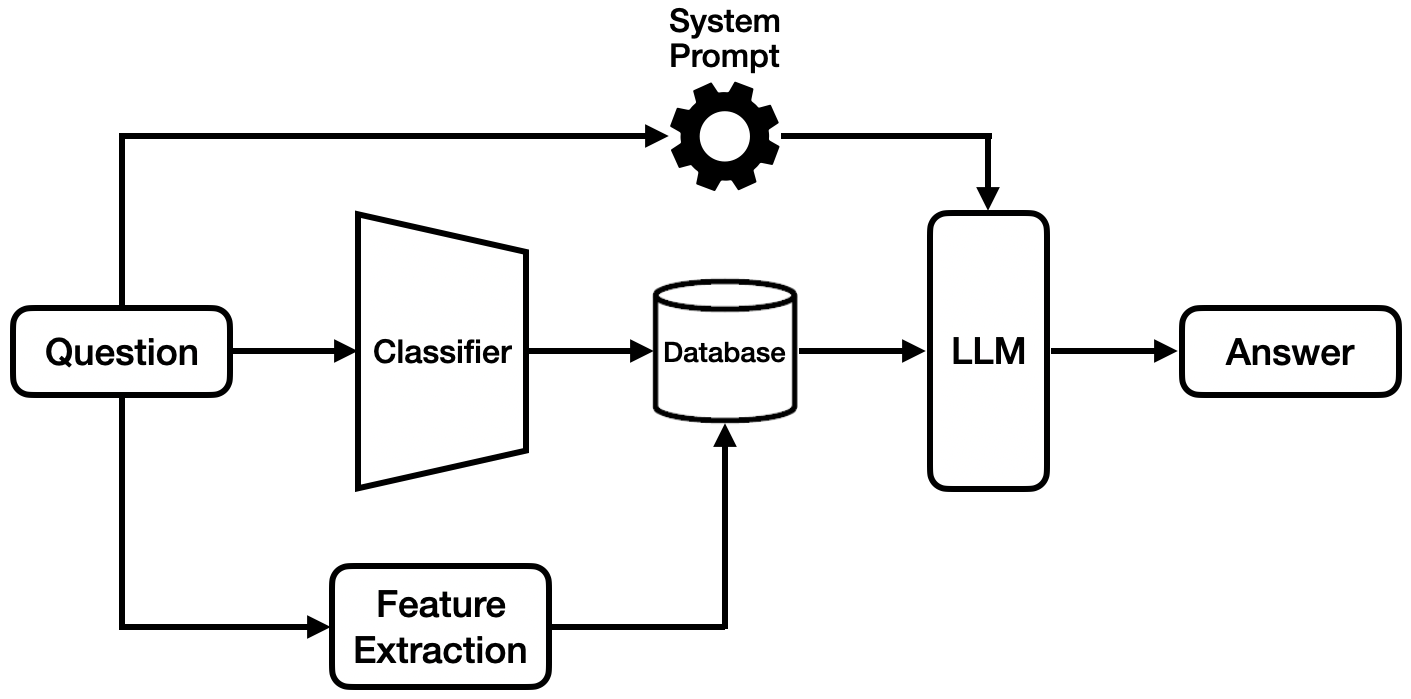
\includegraphics[width=0.60\linewidth]{assets/crg_diagram.png}
    \caption{Classify-Retrieve-Generate (CRG) Pipeline}
    \label{fig:crg_flow}
\end{figure*}

Question and answer pairs were human-generated, ensuring accuracy and eliminating the risk of misinformation.
To expand the dataset and improve generalization, data augmentation techniques were employed.
This included paraphrasing questions, rephrasing answers, and introducing synonyms to create variations of the original pairs.
To efficiently augment the dataset, each question answer pair was fed into ChatGPT to generate multiple variations of the same question and answer.

The dataset is stored in the SQuAD format \cite{b7}. 
The SQuAD format includes a list of topics as the top level, with each topic having a title. 
In each topic exist paragraphs, these contain context to the topic and question-answer pairs.
To fit the dataset to the task at hand, the topics were chosen based off of types of questions that could be asked about the department:
degree programs, research opportunities, facilities and resources, clubs and organizations, career opportunities, internships, financial aid and scholarships, faculty information, admission process, and location and contact.

The dataset consists of 421 question-answer pairs, with 10 categories.
A table summarizing the dataset can be seen in Table \ref{tab:dataset}.
\begin{table}[h]
    \centering
    \caption{Custom Dataset Summary}
    \begin{tabular}{|c|c|}
        \hline
        \textbf{Category} & \textbf{Number of Pairs} \\ \hline
        Degree Programs & 55 \\ \hline
        Research Opportunities & 77 \\ \hline
        Facilities and Resources & 85 \\ \hline
        Clubs and Organizations & 71 \\ \hline
        Career Opportunities & 60 \\ \hline
        Internships & 25 \\ \hline
        Financial Aid and Scholarships & 39 \\ \hline
        Faculty Information & 0 \\ \hline
        Admission Process & 0 \\ \hline
        Location and Contact & 9 \\ \hline
    \end{tabular}
    \label{tab:dataset}
\end{table}

%== DirectLLM Model ==%
\section{DirectLLM Model}
\subsection{Model Selection and Justification}
The DirectLLM model consists of a pre-trained LLM that is fine-tuned on the custom dataset.
To meet the project's objectives, the language model was developed with the following criteria in mind: it had to be open source, capable of effective training on both question-and-answer (Q\&A) datasets and web page content, and optimized for lightweight deployment with quick response times on a microcontroller platform.

An open-source language model was chosen due to their capabilities in lightweight implementations while maintaining high-quality natural language understanding and generation.
Open-source models such as FLAN-T5 \cite{b8} and BART \cite{b9} provide a solid foundation due to their small size and performance on Q\&A task with minimal fine-tuning. 
These models are well-suited for customization and can be fine-tuned with domain-specific data.

Fine-tuned Langauge Agnostic Network (FLAN-T5) is a variant of the T5 (Text-to-Text Transfer Transformer) model, which is pretrained on a diverse range of tasks. 
It features strong ability to be trained on a wide variety of datasets, including Q\&A tasks. 
It also meets the versatile, scalability, and open-source criteria. 
The model used in this project has 77 million parameters, making it lightweight and suitable for deployment on resource-constrained devices.

Bidirectional and Auto-regressive Transformer (BART) is a sequence-to-sequence model optimized for tasks like text generation, summarization, and translation. 
It combines bidirectional context encoding with autoregressive decoding. 
It features capabilities to fine-tune on specific datasets, and effective in both understanding and generating coherent responses.
Like FLAN-T5, it meets the criteria concerned with being open-source, scalable, and versatile. 
The model used in this project has 139 million parameters, making it suitable for deployment on moderately resource-constrained devices.

\subsection{Training and Fine-Tuning Process} 
Both FLAN-T5 and BART were finetuned on the same custom dataset. The model hyperparameters can be found in Table \ref{tab:hyperparams}.
The test dataset included eight questions pertaining to the CSEE department, topics of the questions including: degree programs, research opportunities, student organizations, and career opportunities. 

\begin{table}[!ht]
    \centering
    \caption{Hyperparameters for FLAN-T5 and BART Fine-Tuning}
    \label{tab:hyperparams}
    \begin{tabular}{l|c|c}
        \toprule
        \textbf{Hyperparameter}         & \textbf{FLAN-T5}         & \textbf{BART} \\
        \midrule
        Evaluation Strategy             & Epoch                   & Epoch                     \\ 
        Weight Decay                    & 0.01                    & 0.01                      \\ 
        Learning Rate                   & 5e-5                    & 3e-5                      \\ 
        Logging Steps                   & 5                       & 5                         \\ 
        Train Batch Size                & 8                       & 8                         \\ 
        Evaluation Batch Size           & 8                       & 8                         \\ 
        Number of Training Epochs       & 10                      & 5                         \\ 
        \bottomrule
    \end{tabular}
\end{table}

\subsection{Deployment on Microcontroller}
The implementation of FLAN-T5 and BART leverages Hugging Face Transformers, a comprehensive framework for working with pre-trained language models.
Training was done via the Hugging Face training pipeline, built on the Trainer class and text generation was configured for inference using the Hugging Face pipeline for text generation.
Each model utilized their own transformer: The T5 Tokenizer \cite{b10} for FLAN-T5 and BART Tokenizer \cite{b11} for BART.

% # TODO: deployment on microcontroller 

% \subsection{Strengths and Limitations}
% % # TODO: strengths and limitations of the model 

%== Classify-Retrieve-Generate (CRG) Model ==%
\section{Classify-Retrieve-Generate (CRG) Model}
To address the issues of how to handle new information in the LCSEE, a new approach is needed. 
Instead of a DirectLLM approach, which would need to be retrained with new information, the classify-retrieve-generate (CRG) approach is proposed. 
The main approach here is to have a neural network classify the question asked into the type of question (i.e. degree programs, research, etc) with some encoded information to look up the answer in a database. 
Once fetched, the raw data is fed into a basic LLM that will refine the response to a more natural response.
The CRG pipeline can be seen in Figure \ref{fig:crg_flow}.

\subsection{Classification Step}
To initiate the CRG pipeline, a classifier is used to determine the category of an incoming question. 
Each category corresponds to a high-level topic (e.g., degree programs, research opportunities) within the LCSEE department's offerings
Several classification approaches were explored, ranging from traditional machine learning to transformer-based fine-tuned models. 
In each approach, the input question is first transformed into a numerical format using Term Frequency–Inverse Document Frequency (TF-IDF), word embeddings, or contextual token embeddings.

\subsubsection{Traditional Machine Learning Approaches}
\textbf{Logistic Regression for Multi-Class Classification:}
Logistic regression is a linear model that predicts the probability distribution over a set of classes using a softmax function. 
It is particularly well-suited for structured, lower-dimensional feature spaces such as TF-IDF vectors.

Given an input feature vector $\mathbf{x}\in \mathbb{R}^n$, the probability of class $i\in{1,2,\ldots,k}$ is given by:
\begin{equation}
    P(y_i | \mathbf{x}) = \frac{e^{\beta_i^T \mathbf{x}}}{\sum_{j=1}^{k} e^{\beta_j^T \mathbf{x}}}
\end{equation}
where $\beta_i$ is the weight vector for class $i$, and $k$ is the number of classes.
Training involves minimizing the cross-entropy loss between the predicted and actual distributions.
\begin{equation}
    \mathcal{L}_{CE} = -\sum_{i=1}^{k} y_i \log(P(y=i | \mathbf{x}))
\end{equation}

TF-IDF is used to convert questions into vector representations before being fed into the classifier.
The term frequency $\text{TF}(t)$  and the inverse document frequency $\text{IDF}(t)$ are defined as:
\begin{equation}
    \text{TF}(t) = \frac{f_{t,d}}{\sum_{t' \in d} f_{t',d}}
\end{equation}
\begin{equation}
    \text{IDF}(t) = \log\left(\frac{N}{|\{d \in D: t \in d\}|}\right)
\end{equation}
where $f_{t,d}$ is the frequency of term $t$ in document $d$, $N$ is the total number of documents, and $D$ is the set of all documents.
The TF-IDF vector for a term $t$ in document $d$ is given by:
\begin{equation}
    \text{TF-IDF}(t) = \text{TF}(t) \cdot \text{IDF}(t)
\end{equation}
This method is fast and computationally efficient, making it a strong baseline for classification tasks with small to medium-sized datasets.

\textbf{Support Vector Machines (SVM):}
SVMs are another traditional method that finds a hyperplane to separate classes by maximizing the margin. 
In the multi-class setting, a One-vs-Rest (OvR) strategy is typically employed. 
The decision function for each class is defined as:
\begin{equation}
    f_i(\mathbf{x}) = \sum_{i=1}^{k} \mathbf{w}^T_i \mathbf{x} + b_i
\end{equation}
where $\mathbf{w}_i$ is the learned weight vector for class $i$, and $b_i$ is the bias term.
The predicted class is:
\begin{equation}
    \hat{y} = \arg\max_{i} f_i(\mathbf{x})
\end{equation}
SVMs use the hinge loss function to enforce a margin between decision boundaries:
\begin{equation}
    \mathcal{L}_{hinge} = \sum_{i=1}^{k} \max(0, 1 - y_i f_i(\mathbf{x}))
\end{equation}
These models work well when the data is not deeply contextual, and they offer high speed and generalization performance for TF-IDF inputs.

\subsubsection{Transformer-Based Classification}
\textbf{BERT (Bidirectional Encoder Representations from Transformers):}
BERT is a transformer-based model pretrained on large corpora using masked language modeling \cite{b12}. 
It captures contextual relationships in text by processing input bidirectionally. 
For classification, the [CLS] token's embedding is used and passed through a feedforward classifier layer. 
The model is fine-tuned on the task-specific dataset, with the SQuAD-like format providing labeled classes for supervised training.

Fine-tuning BERT involves updating all transformer weights using a small learning rate and minimizing cross-entropy loss over the predicted class probabilities. 
While BERT achieves high accuracy, it is computationally heavy and slower during inference, which can be problematic for edge or real-time applications.

\textbf{DistilBERT:}
DistilBERT is a lighter and faster version of BERT, trained via knowledge distillation \cite{b13}. 
It retains about 97\% of BERT's performance while being 60\% faster and using 40\% fewer parameters. 
Like BERT, the classification token is used to predict the question category, and the model is fine-tuned on the custom dataset.

DistilBERT offers a balance between performance and efficiency, making it suitable for mobile or embedded systems where fast inference is critical.

A comparative summary of the classification methods is presented in Table \ref{tab:classification_comparison}.
These models were all trained and tested on the same labeled dataset of questions and categories. 
Evaluation metrics such as accuracy, F1 score, and response time are discussed in Section \ref{sec:evaluation}.

\begin{table}[!ht]
    \centering
    \caption{Comparative Summary of Classification Models}
    \label{tab:classification_comparison}
    \begin{tabular}{l|l|l}
        \toprule
        \textbf{Model}         & \textbf{Accuracy}         & \textbf{Inference Speed} \\
        \midrule
        Logistic Regression & Medium & Fast \\
        Support Vector Machine & High & Fast \\
        BERT                & Very High & Slow \\
        DistilBERT          & High & Medium \\
        \bottomrule
    \end{tabular}
\end{table}

\subsection{Feature Extraction Techniques}
In the CRG pipeline, once a question is classified into a specific category (e.g., research opportunities, clubs and organizations), the next step is to extract meaningful features from the question to assist in retrieving the most relevant answer. 
Since each category may contain numerous similar question-answer pairs, surface-level classification alone is insufficient. 
This section outlines three primary methods explored for extracting relevant information from user queries: Named Entity Recognition (NER), TF-IDF keyword extraction, and word embeddings for semantic search.

\subsubsection{Named Entity Recognition (NER)}
Named Entity Recognition (NER) is a technique used to identify and label key terms in a sentence that refer to proper nouns, such as names of people, organizations, degrees, or locations. 
For this project, spaCy's pretrained NER model \cite{b14} was employed to identify relevant entities within user queries. For example, in the question:

\begin{quote}
    ``What research is done in the biometrics field?''
    
    NER extracts: \textit{research}, \textit{biometrics}, \textit{field} 
\end{quote}

\begin{quote}
    ``What dual degrees can I pursue?''
    
    NER extracts: \textit{degree} 
\end{quote}

This method performs well when questions contain distinct, recognizable entities (e.g., Cybersecurity, Morgantown, Capstone), but may struggle with abstract or compound terms (e.g., dual degree, interdisciplinary program). 
Additionally, the pretrained models are not optimized for the specific academic domain, leading to inconsistent coverage of niche terminology.

\subsubsection{TF-IDF Keyword Extraction}
TF-IDF can also be applied to extract high-value keywords from a question. 
It assigns each word a score indicating its importance in the current question relative to a background corpus.

\begin{quote}
    ``What research is done in the biometrics field?''
    
    NER extracts: \textit{research}, \textit{biometrics}, \textit{field} 
\end{quote}

\begin{quote}
    ``What dual degrees can I pursue?''
    
    NER extracts: \textit{dual}, \textit{degree}, \textit{pursue}
\end{quote}
This technique is computationally lightweight and works well with short inputs like student queries. 
However, its primary limitation is a lack of semantic awareness; it treats each word independently and cannot recognize synonyms or related phrases. 
For instance, questions about "job prospects" and "career opportunities" may score very differently even if they refer to the same concept.

\subsubsection{Word Embeddings for Semantic Search} \label{sec:word_embeddings}
To overcome the limitations of sparse keyword methods, semantic embeddings are used to convert entire questions into dense vector representations.
The \textit{all-MiniLM-L6-v2} model from Sentence Transformers \cite{b15} \cite{b16} was chosen for this purpose, as it provides high-quality sentence embeddings that capture semantic meaning effectively.
The model generates a 384-dimensional vector for each input question, where semantically similar questions are closer in the vector space.

This method yields the best retrieval results in cases where questions are phrased ambiguously or contain rare synonyms. 
However, it is computationally more expensive than NER or TF-IDF extraction and requires dimensionality reduction or vector indexing to maintain efficiency in larger datasets

\subsection{Retrieval Methods}
Once a question has been classified and its key features extracted, the next step in the CRG pipeline is to retrieve the most relevant answer from the custom question-answer (Q\&A) dataset. 
The retrieval component compares the incoming query—represented via keywords or vector embeddings—against existing questions in the dataset filtered by category. 
Several techniques were evaluated for this purpose, ranging from simple keyword-based matching to semantic similarity scoring. 
This section outlines the retrieval methods implemented and the mathematical formulations behind them.

\subsubsection{Exact Keyword Intersection (EKI)}
In the EKI method, the set of extracted keywords from the user query is compared to the keywords in each candidate question (within the same classified category). 
Each keyword match is given a score of 1, and the total intersection score is used to rank candidates.
Let $A$ be the set of keywords from the user query, and $B_i$ be the set of keywords from the $i^{th}$ candidate question.
The intersection score is defined as:
\begin{equation}
    \text{EKI}(A, B_i) = |A \cap B_i| 
\end{equation}
The question with the highest EKI score is selected. 
In case of a tie, the first candidate is returned or one is randomly selected. 
While EKI is fast and easy to implement, it is sensitive to exact word matches and ignores synonyms or paraphrasing.

\subsubsection{Jaccard Similarity}
The Jaccard index is a set-based similarity measure used to assess the overlap between two sets of keywords. 
Unlike EKI, it accounts for both shared and distinct elements.
The Jaccard score between sets $A$ and $B_i$ is defined as:
\begin{equation}
    \text{Jac}(A, B_i) = \frac{|A \cap B_i|}{|A \cup B_i|}
\end{equation}
This score ranges from 0 (no overlap) to 1 (complete match). 
The candidate with the highest Jaccard score is chosen. 
Ties are handled similarly to EKI. 
Jaccard provides better granularity than raw intersection and is more robust for uneven keyword set.

\subsubsection{JEKI Score (Jaccard + EKI Hybrid)}
To combine the strengths of EKI and Jaccard, a weighted score called the JEKI score was introduced:
\begin{equation}
    \text{JEKI}(A, B_i) = \lambda \cdot \text{EKI}(A, B_i) + (1 - \lambda) \cdot \text{Jac}(A, B_i)
\end{equation}
where $\lambda \in [0, 1]$ is a hyperparameter that balances the two components.

This hybrid approach improves answer selection, especially in tie cases where EKI or Jaccard alone yields similar scores. 
The balance between raw match count and normalized similarity allows JEKI to adapt across diverse query styles.

\subsubsection{Vector Space Retrieval via Cosine Similarity}
For a more semantic retrieval method, user queries and candidate questions can be encoded into dense vector embeddings using pretrained models (as described in Section \ref{sec:word_embeddings}). 
These vectors are compared using cosine similarity, defined as:
\begin{equation}
    \cos(\theta) = \frac{ \vec{q} \cdot \vec{q}_i }{ ||\vec{q}|| \cdot ||\vec{q}_i|| }
\end{equation}
where $\vec{q}$ is the vector for the user query and $\vec{q}_i$ is the vector for the $i^{th}$ candidate question.

The question with the highest cosine similarity is retrieved. 
This method captures contextual closeness even when wording differs significantly (e.g., "student groups" vs. "clubs and organizations"). 
It requires more memory and computation but yields the highest retrieval accuracy in semantically diverse queries.

\subsection{Generation Step}
The final step in the CRG (Classify-Retrieve-Generate) pipeline is the generation stage, which takes the retrieved answer and rephrases it into a more natural, engaging, and conversational response. 
This layer transforms a static Q\&A system into a dynamic tour experience, simulating human-like dialogue. 
Rather than relying on a large end-to-end model like in the DirectLLM approach, this modular step uses lightweight generation models tailored for refinement, not inference.

The inputs to the generation model include: the original user query, the retried answer, and a system prompt that defines the tone and style of the assistant.
The generation model is prompted to use the retrieved answer directly, then follow it up with a question or elaboration to encourage ongoing interaction. 
A sample system prompt used in experimentation was:

\begin{quote}
    "You are an AI assistant for a university tour guide. 
    Your role is to provide engaging and helpful responses based on the retrieved answer. 
    You must always use the retrieved answer in your response first. 
    Then, ask a relevant follow-up question to encourage further conversation."
\end{quote}

Several small-scale generative models were tested for compatibility with edge devices.
FLAN-T5: Instruction-tuned, lightweight transformer. Easy to deploy but struggles with prompt adherence at smaller sizes.
TinyLlama (1.1B): Small, instruction-following model showing early promise in producing coherent responses with minimal compute.
DistilBERT: Evaluated but rejected—lacks generative capabilities.
GPT-Neo and Mistral-7B: Tested for baseline comparison; too large for final deployment.

All models were run with variations in system prompts and temperature settings to observe response variability and coherence.
This step remains work-in-progress. 
Preliminary results show inconsistent behavior in prompt adherence—many models fail to include the retrieved answer or ask relevant follow-up questions. 
Further fine-tuning and prompt engineering are planned.

\begin{table}[h]
    \centering
    \caption{Summary of Response Generation Models (Preliminary)}
    \begin{tabular}{l|c|c|c}
    \hline
    \textbf{Model} & \textbf{Params} & \textbf{Output Quality} & \textbf{Edge Suitability} \\
    \hline
    FLAN-T5-Small & 80M & Inconsistent & High  \\
    TinyLlama & 1.1B & Promising & High  \\
    GPT-Neo & 1.3B & Mixed & Medium  \\
    Mistral-7B & 7B & High & Low  \\
    \hline
    \end{tabular}
    \label{tab:generation_models}
\end{table}

%== Evaluation and Comparison ==%
\section{Evaluation and Comparison} \label{sec:evaluation}
This section compares the performance of the DirectLLM approaches and the CRG approaches in addressing question about the LCSEE department.
The evaluation framework considers both quantitative metrics (accuracy, F1, BLEU, response time) and qualitative observations (response fluency, robustness, ease of update).
\subsection{DirectLLM Evaluation}
To evaluate the performance of FLAN-T5 and BART, two metrics are employed: F1 Score and BLEU score. 
These metrics provide insight to the models' precision, recall, and accuracy in text understanding and generation tasks.
Another metric used to evaluate the model is average response time, or the mean of the time it takes to process an input and provide an output over all test data.

\noindent
\textbf{F1 Score:}
The F1 Score is a harmonic mean of precision and recall, offering a single metric to evaluate a model's ability to balance false positives and false negatives.
The calculation for the F1 Score is seen in Equation \ref{eq:F1}.

\begin{equation} \label{eq:F1}
    \text{F1} = 2 \cdot \frac{P \cdot R}{P + R}
\end{equation}
where $P$ is the precision and $R$ is the recall over the test dataset. 

\noindent
\textbf{BLEU Score:}
The Bilingual Evaluation Understudy (BLEU) Score measures the quality of the text generated by comparing it with one or more of the reference texts.
It assesses how similar the generated text is to human-provided references, in this case the reference is the provided answer to the test question. 
The BLEU Score formula is seen in Equation \ref{eq:BLEU}.

\begin{equation} \label{eq:BLEU}
    \text{BLEU} = \text{BP} \cdot \exp \left( \sum_{n=1}^{N} w_n \log(p_n) \right)
\end{equation}
\begin{equation} \label{eq:BP}
    \text{BP} = 
    \begin{cases}
        1, & c > r \\
        e^{1 - r/c}, & c \leq r
    \end{cases}
\end{equation}
\noindent
where $\text{BP}$ is the Brevity Penalty (seen in Equation \ref{eq:BP}), $p_n$ is the precision of $n$-grams, and $w_n$ is the weight associated to $n$-grams (typically equal $\forall n$).

\subsection{CRG Evaluation}
The various combinations of implementations for each step in the CRG pipeline were evaluated to determine their effectiveness in answering questions about the LCSEE department.
In total there are 96 combinations of the CRG pipeline, the best three combinations are shown in this section. 
Table \ref{tab:crg_combinations} summarizes the three best-performing CRG configurations, including the classification model, retrieval method, and generation model used in each case.

\begin{table}[!ht]
    \centering
    \caption{Best Performing CRG Combinations}
    \label{tab:crg_combinations}
    \begin{tabular}{l|l|l|l}
        \toprule
        \textbf{CRG Model} & \textbf{Classification} & \textbf{Extraction} & \textbf{Retrieval} \\
        \midrule
        CRG-1 & LR & Vector & Cosine \\
        CRG-2 & SVM & NER & EKI \\
        CRG-3 & DistilBERT & Vector & Cosine \\
        \bottomrule
    \end{tabular}
\end{table}

The classification is evaluated on accuracy, which is the ratio of correctly classified questions to the total number of questions in the test set.
The retrieval is evaluated using a retrieval score ($\text{RS}$), which is a binary score indicating where the correct answer was retrieved from the dataset. 
\begin{equation}
    \text{RS} = \frac{1}{N} \sum_{i=1}^{N} \mathbb{I}(y_i = \hat{y}_i)
\end{equation}

Both DirectLLM and CRG are evaluated by their mean response time over the test dataset.
The DirectLLM results are seen in Table \ref{tab:directllm_results}, while the CRG results are seen in Table \ref{tab:crg_results}.

\begin{table}[!ht]
    \centering
    \caption{DirectLLM Evaluation}
    \label{tab:directllm_results}
    \begin{tabular}{l|c|c|c}
        \toprule
        \textbf{Model} & \textbf{F1 (\%)} & \textbf{BLEU Score (\%)} & \textbf{Avg. Resp. Time (s)} \\
        \midrule
        FLAN-T5        & 36.094                 & 74.275                   & 0.976                          \\
        BART           & 40.546                 & 80.402                   & 1.442                          \\
        \bottomrule
    \end{tabular}
\end{table}

\begin{table}[!ht]
    \centering
    \caption{CRG Evaluation}
    \label{tab:crg_results}
    \begin{tabular}{l|c|c|c}
        \toprule
        \textbf{Model} & \textbf{Class Accuracy (\%)} & \textbf{RS} & \textbf{Avg. Resp. Time (s)} \\
        \midrule
        CRG-1 & 85.71 & 0.875 & 1.798 \\
        CRG-2 & 71.43 & 0.429 & 0.518 \\
        CRG-3 & 75.00 & 0.750 & 2.215 \\
        \bottomrule
    \end{tabular}
\end{table}

Sample outputs from both DirectLLM and CRG models can be found in Appendix \ref{app:directllm_output} and \ref{app:crg_output}, respectively.

%== Discussion ==%
\section{Discussion}
\subsection{Lessons Learned}
Through the development and evaluation of both the DirectLLM and Classify-Retrieve-Generate (CRG) approaches, several key insights emerged regarding their suitability for deployment in a robotic tour guide system.

One of the primary challenges with the DirectLLM pipeline was the training bottleneck imposed by dataset requirements. 
As a fine-tuned small language model (SLM), DirectLLM demands a substantial and diverse dataset to maintain conversational accuracy across a wide range of questions. 
Furthermore, any updates to department-specific information (e.g., new faculty, facilities, or programs) would necessitate retraining the entire model. 
This approach is neither scalable nor maintainable for dynamic environments, particularly when operating on constrained hardware.

In contrast, the CRG framework introduced a modular alternative. 
By decoupling classification, retrieval, and generation into distinct steps, CRG enables individual components to be updated or replaced without the need to retrain an end-to-end model. 
For example, new answers can be added directly to the retrieval database without affecting the classifier or generator. 
This modularity makes CRG especially well-suited for educational deployments where content frequently evolves.

\subsection{Trade-Offs}
While CRG offers clear advantages in adaptability and maintainability, it comes with certain trade-offs. 
DirectLLM, once trained, can provide highly fluent and contextually rich responses, particularly for open-ended questions. 
The model leverages deep contextual embeddings to infer nuanced intent and generate more natural responses.

However, this fluency comes at the cost of scalability and update flexibility. 
CRG, though more structured and sometimes less fluent in response style, allows for deterministic output based on a well-controlled retrieval mechanism. 
Additionally, CRG's modular design permits fine-grained improvements to individual components such as classification accuracy or retrieval algorithms without affecting the entire pipeline.

\subsection{Practical Considerations}
For deployment on microcontroller-based robots, several practical considerations must be addressed. 
Inference time and memory usage are critical constraints. 
DirectLLM models, such as BART and FLAN-T5, exhibited slower average response times and higher memory footprints. 
In contrast, the CRG system, particularly when using lightweight models like Logistic Regression or DistilBERT for classification, offered significantly faster and more deterministic performance, making it a better fit for real-time conversational interactions on low-power hardware.

Furthermore, CRG's deterministic logic and rule-based fallback mechanisms enhance its reliability, which is crucial in educational contexts where incorrect or hallucinated responses could erode user trust.

\section{Conclusion}
This research presented the development of an AI-powered robotic tour guide for the Lane Department of Computer Science and Electrical Engineering (LCSEE), leveraging two natural language processing (NLP) pipelines: DirectLLM and Classify-Retrieve-Generate (CRG). 
Each approach was designed, implemented, and evaluated with the goal of enabling natural, accurate, and efficient interactions between prospective students and the department's offerings.

The DirectLLM approach demonstrated strong performance in generating fluent and context-rich responses, benefiting from end-to-end fine-tuning on a curated dataset. 
However, this pipeline faces a critical training bottleneck: any update to the departmental information requires full model retraining, making it inefficient and unsuitable for dynamic content environments.

In contrast, the CRG pipeline offers a modular architecture that separates classification, retrieval, and generation into discrete components. 
This separation enables more efficient updates—new content can be added directly to the retrieval database without retraining. 
CRG also supports targeted tuning of individual components such as the classifier or generator, improving maintainability and adaptability for evolving informational needs.

Despite its flexibility, CRG faces its own challenges, particularly in ensuring the fluency and coherence of generated responses. 
The system still requires improvements in response generation fidelity and optimization for real-time usage.

\subsection*{Future Work}
To enhance the robustness and usability of the tour guide system, several directions are proposed for future research:
Expand the custom dataset with more diverse and detailed question-answer pairs to improve both DirectLLM and CRG coverage.
Finish development of the CRG generation step, ensuring it reliably incorporates retrieved answers and poses engaging follow-up questions.
Further fine-tune the DirectLLM models, particularly BART and FLAN-T5, using the expanded dataset to improve their fluency and domain-specific relevance.
Improve classification accuracy in the CRG pipeline, which involves further fine-tuning.
Optimize code efficiency in each CRG stage, especially in retrieval and generation, to meet real-time requirements on embedded hardware.
Explore hybrid fusion models that combine the strengths of both pipelines—such as using CRG for structured queries and DirectLLM for free-form conversational fallback—to balance performance and flexibility.
Together, these enhancements aim to advance the system toward a fully autonomous, scalable, and engaging AI tour guide platform deployable across academic institutions.

\begin{thebibliography}{00}
\bibitem{b1} Mangdang, "Mangdang Store," Available: https://mangdang.store
\bibitem{b2} M. Rajkomar et al., "Scalable and accurate deep learning with electronic health records," npj Digital Medicine, vol. 1, no. 18, 2018.
\bibitem{b3} T. Dettmers et al., "Sparse fine-tuning for efficient deployment of large-scale language models," NeurIPS Conference Proceedings, 2022.
\bibitem{b4} Z. Jiang et al., "Efficient deep learning inference on edge devices: Challenges and techniques," ACM Computing Surveys, vol. 55, no. 6, 2023.
\bibitem{b5} H. Touvron et al., "Llama 2: Open foundation and fine-tuned chat models," arXiv:2307.09288, 2023.
\bibitem{b6} Poppy Project, "Poppy Humanoid," Available: https://www.poppy-project.org/en/robots/poppy-humanoid/.
\bibitem{b7} R. Rajpurkar, "SQuAD: The Stanford Question Answering Dataset," SQuAD Explorer.
\bibitem{b8} Chung, Hyung Won, Le Hou, Shayne Longpre, Barret Zoph, Yi Tay, William Fedus, Eric Li, et al. "Scaling Instruction-Finetuned Language Models." arXiv (2022). https://doi.org/10.48550/arXiv.2210.11416.
\bibitem{b9} M. Lewis, Y. Liu, N. Goyal, M. Ghazvininejad, A. Mohamed, O. Levy, V. Stoyanov, and L. Zettlemoyer, "BART: Denoising Sequence-to-Sequence Pre-training for Natural Language Generation, Translation, and Comprehension," CoRR, vol. abs/1910.13461, 2019. [Online]. Available: http://arxiv.org/abs/1910.13461.
\bibitem{b10} H. Xu, M. Scales, A. Nguyen, R. Ritter, C. Raffel, K. Shankar, S. A. Saurous, and Q. V. Le, "Deep Evolutionary Reinforcement Learning," arXiv preprint arXiv:1910.10683, 2019. [Online]. Available: https://arxiv.org/pdf/1910.10683.
\bibitem{b11} M. Lewis, Y. Liu, N. Goyal, M. Ghazvininejad, A. Mohamed, O. Levy, V. Stoyanov, and L. Zettlemoyer, "BART: Denoising Sequence-to-Sequence Pre-training for Natural Language Generation, Translation, and Comprehension," arXiv preprint arXiv:1910.13461, 2019. [Online]. Available: https://arxiv.org/pdf/1910.13461. [Accessed: Dec. 17, 2024].
\bibitem{b12} J. Devlin, M.-W. Chang, K. Lee, and K. Toutanova, “BERT: Pre-training of Deep Bidirectional Transformers for Language Understanding,” arXiv preprint arXiv:1810.04805, 2019. [Online]. Available: https://arxiv.org/abs/1810.04805
\bibitem{b13} V. Sanh, L. Debut, J. Chaumond, and T. Wolf, “DistilBERT, a distilled version of BERT: smaller, faster, cheaper and lighter,” arXiv preprint arXiv:1910.01108, 2020. [Online]. Available: https://arxiv.org/abs/1910.01108
\bibitem{b14} M. Honnibal and I. Montani, "spaCy 2: Natural language understanding with Bloom embeddings, convolutional neural networks and incremental parsing," 2017.
\bibitem{b15} N. Reimers and I. Gurevych, "Making Monolingual Sentence Embeddings Multilingual using Knowledge Distillation," in Proceedings of the 2020 Conference on Empirical Methods in Natural Language Processing (EMNLP), 2020. [Online]. Available: https://arxiv.org/abs/2004.09813
\bibitem{b16} Hugging Face, "all-MiniLM-L6-v2," [Online]. Available: https://huggingface.co/sentence-transformers/all-MiniLM-L6-v2. [Accessed: 01-Apr-2025].
\end{thebibliography}

%-- Appendix --%
\newpage
\onecolumn
\appendix
\section{Appendix}
\subsection{Sample Output from FLAN-T5 and BART} \label{app:directllm_output}
\begin{figure*}[!h]
    \centering
    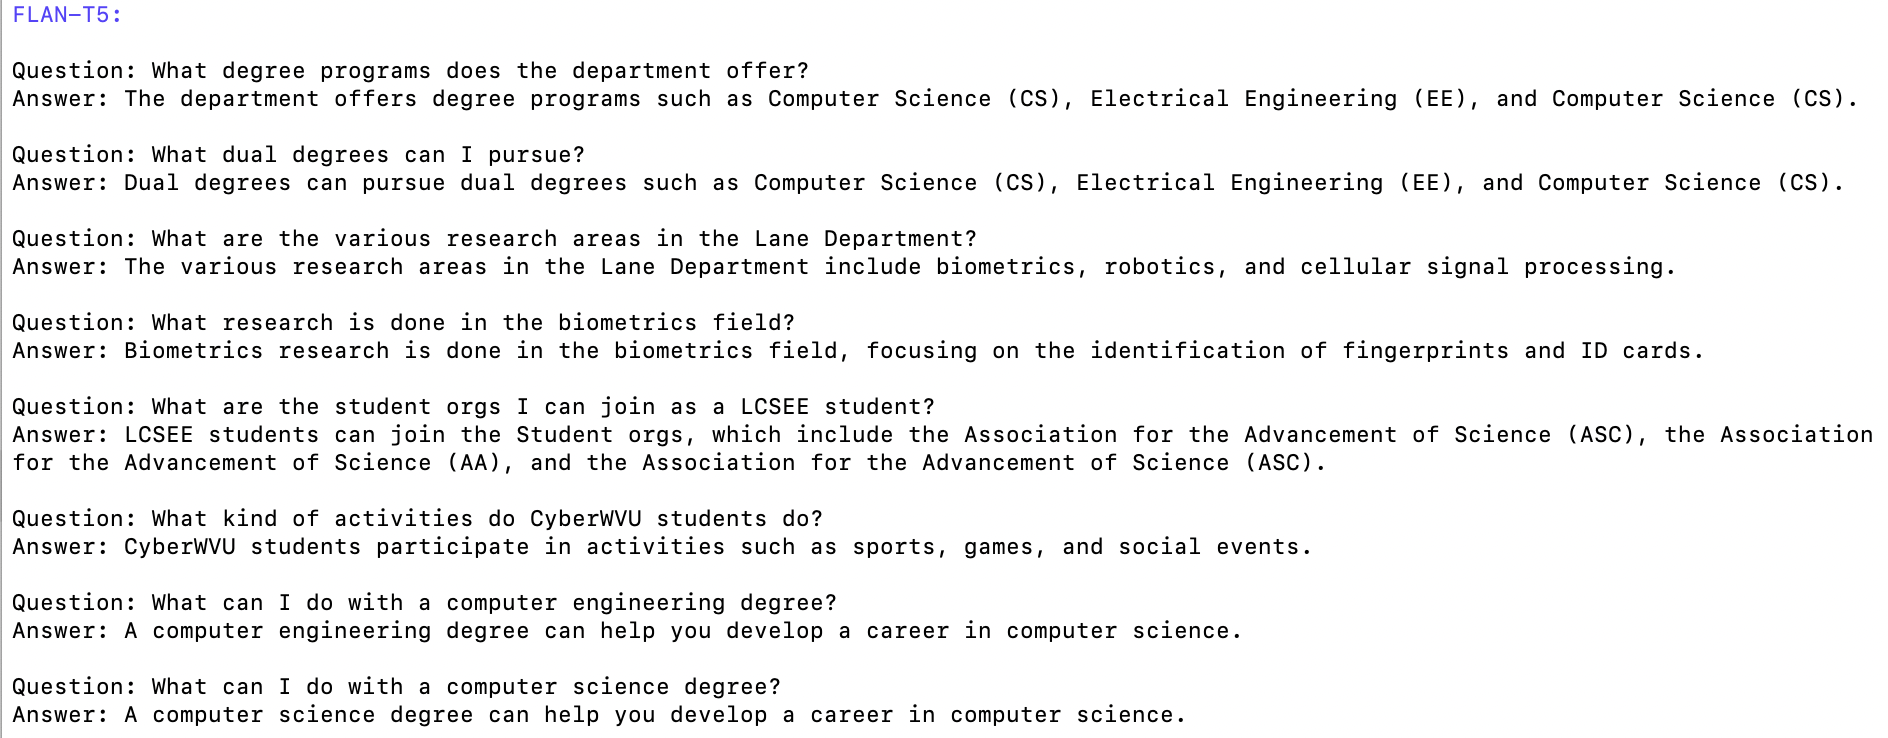
\includegraphics[width=\linewidth]{assets/Flan_out.png}
    \caption{FLAN-T5 Output}
    \label{fig:FLAN_Out}
\end{figure*}

\begin{figure*}[!h]
    \centering
    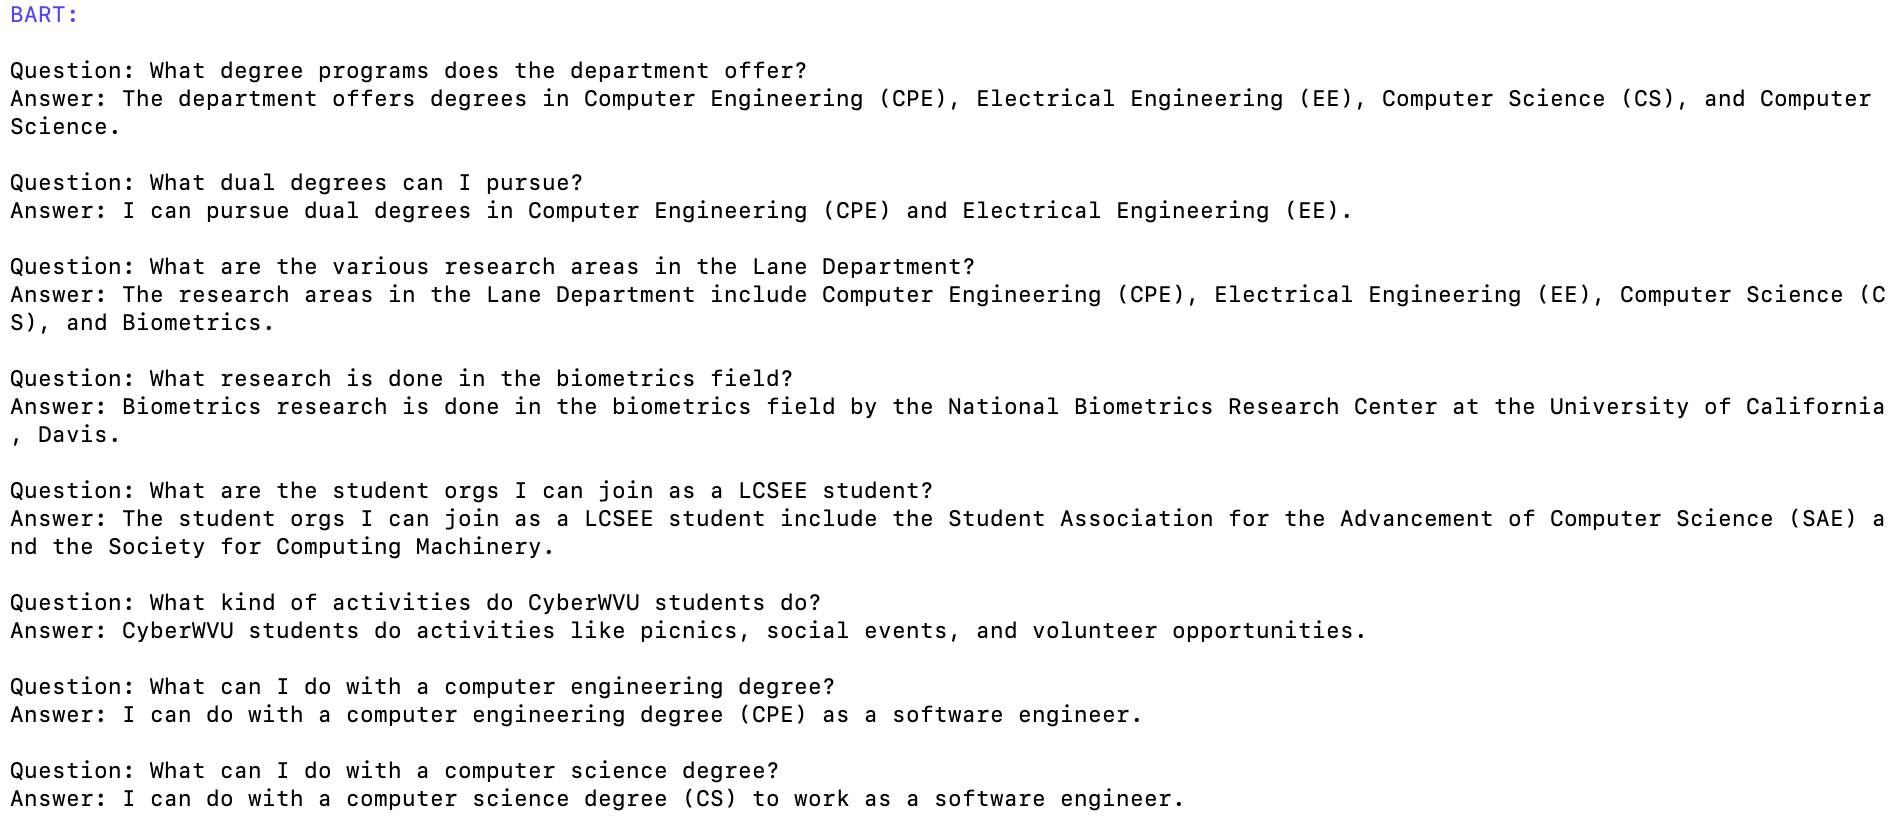
\includegraphics[width=\linewidth]{assets/Bart_out.png}
    \caption{BART Output}
    \label{fig:BART_Out}
\end{figure*}

\newpage
\subsection{Sample Output from CRG} \label{app:crg_output}
\begin{figure*}[!h]
    \centering
    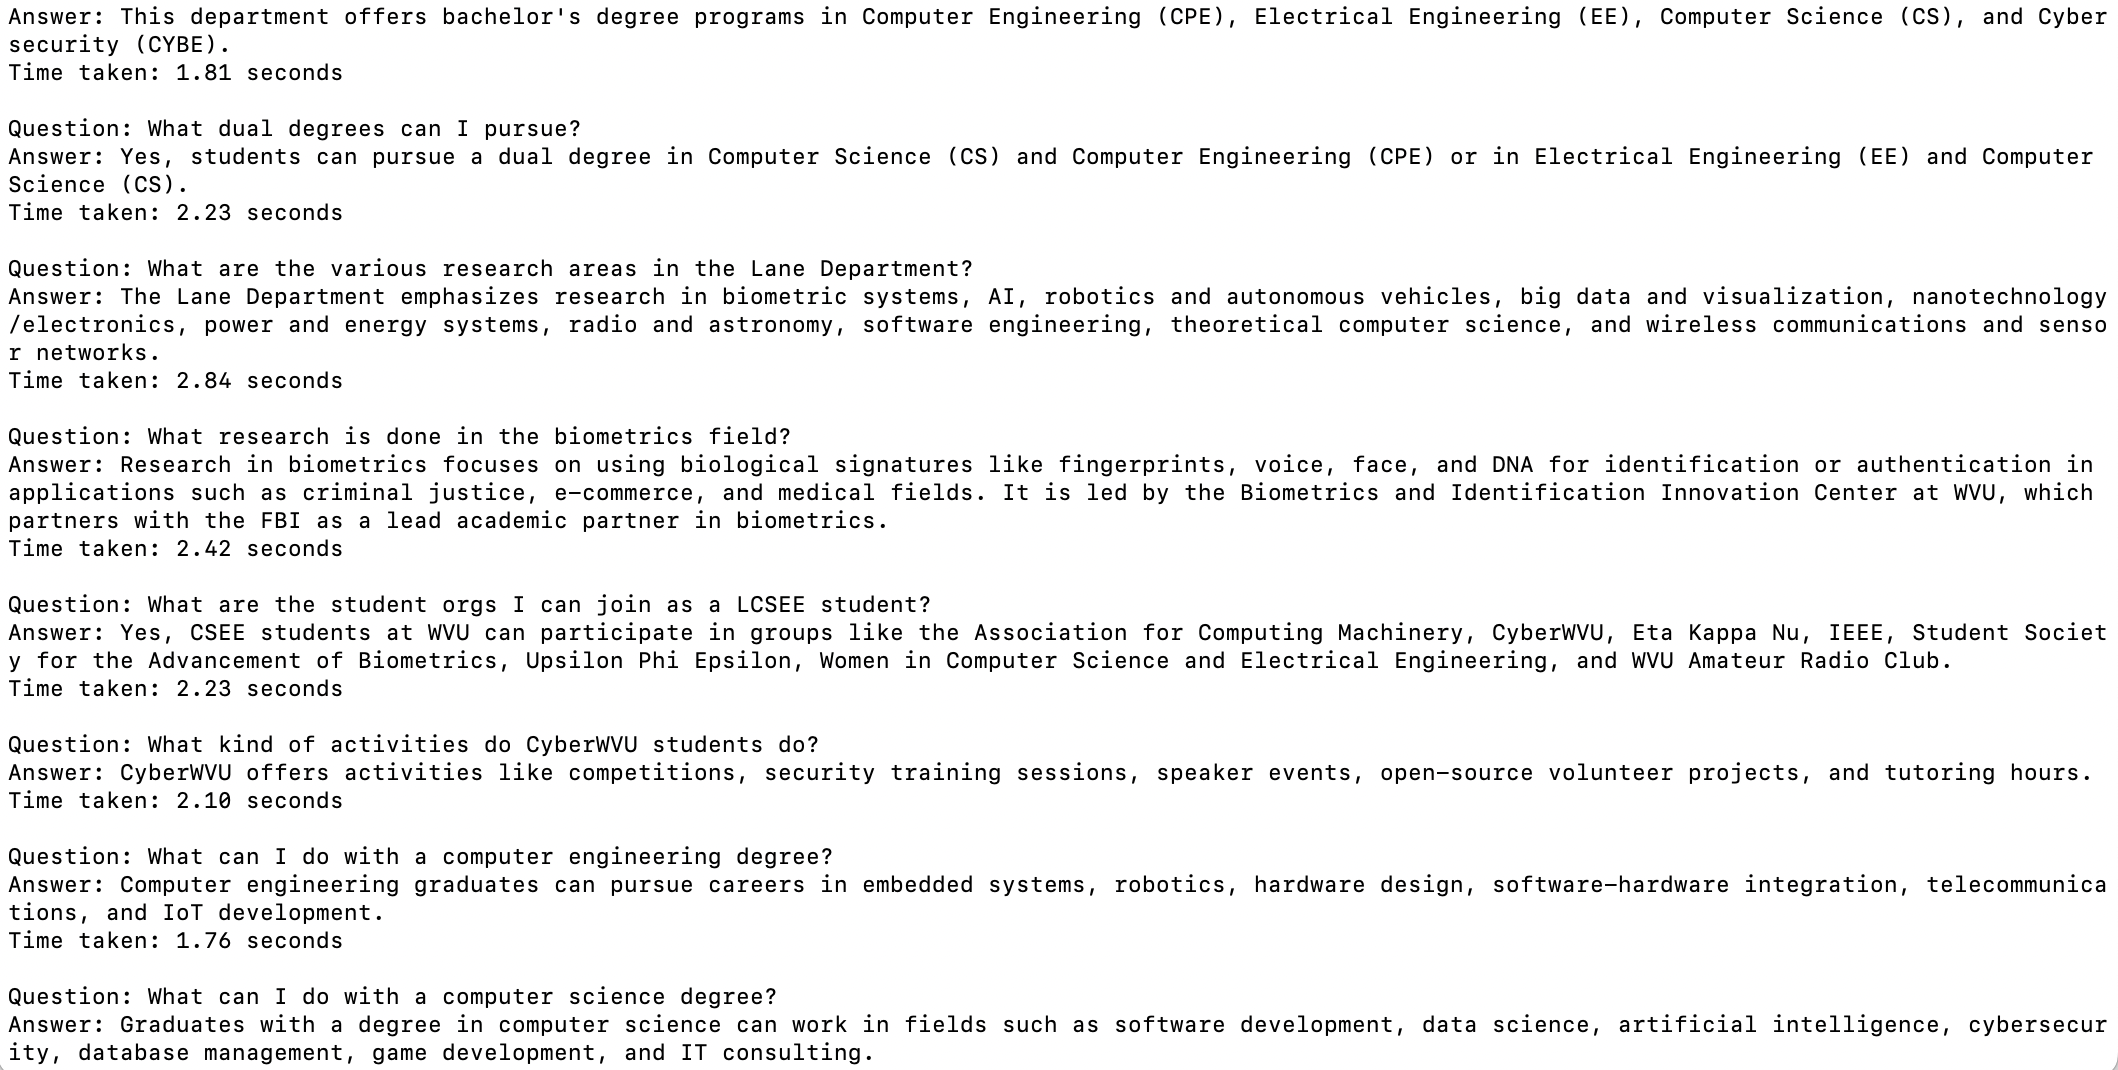
\includegraphics[width=\linewidth]{assets/CRG1_out.png}
    \caption{CRG-1 Output: LR + Vector + Cosine Similarity}
    \label{fig:CRG_1-Out}
\end{figure*}

\begin{figure*}[!h]
    \centering
    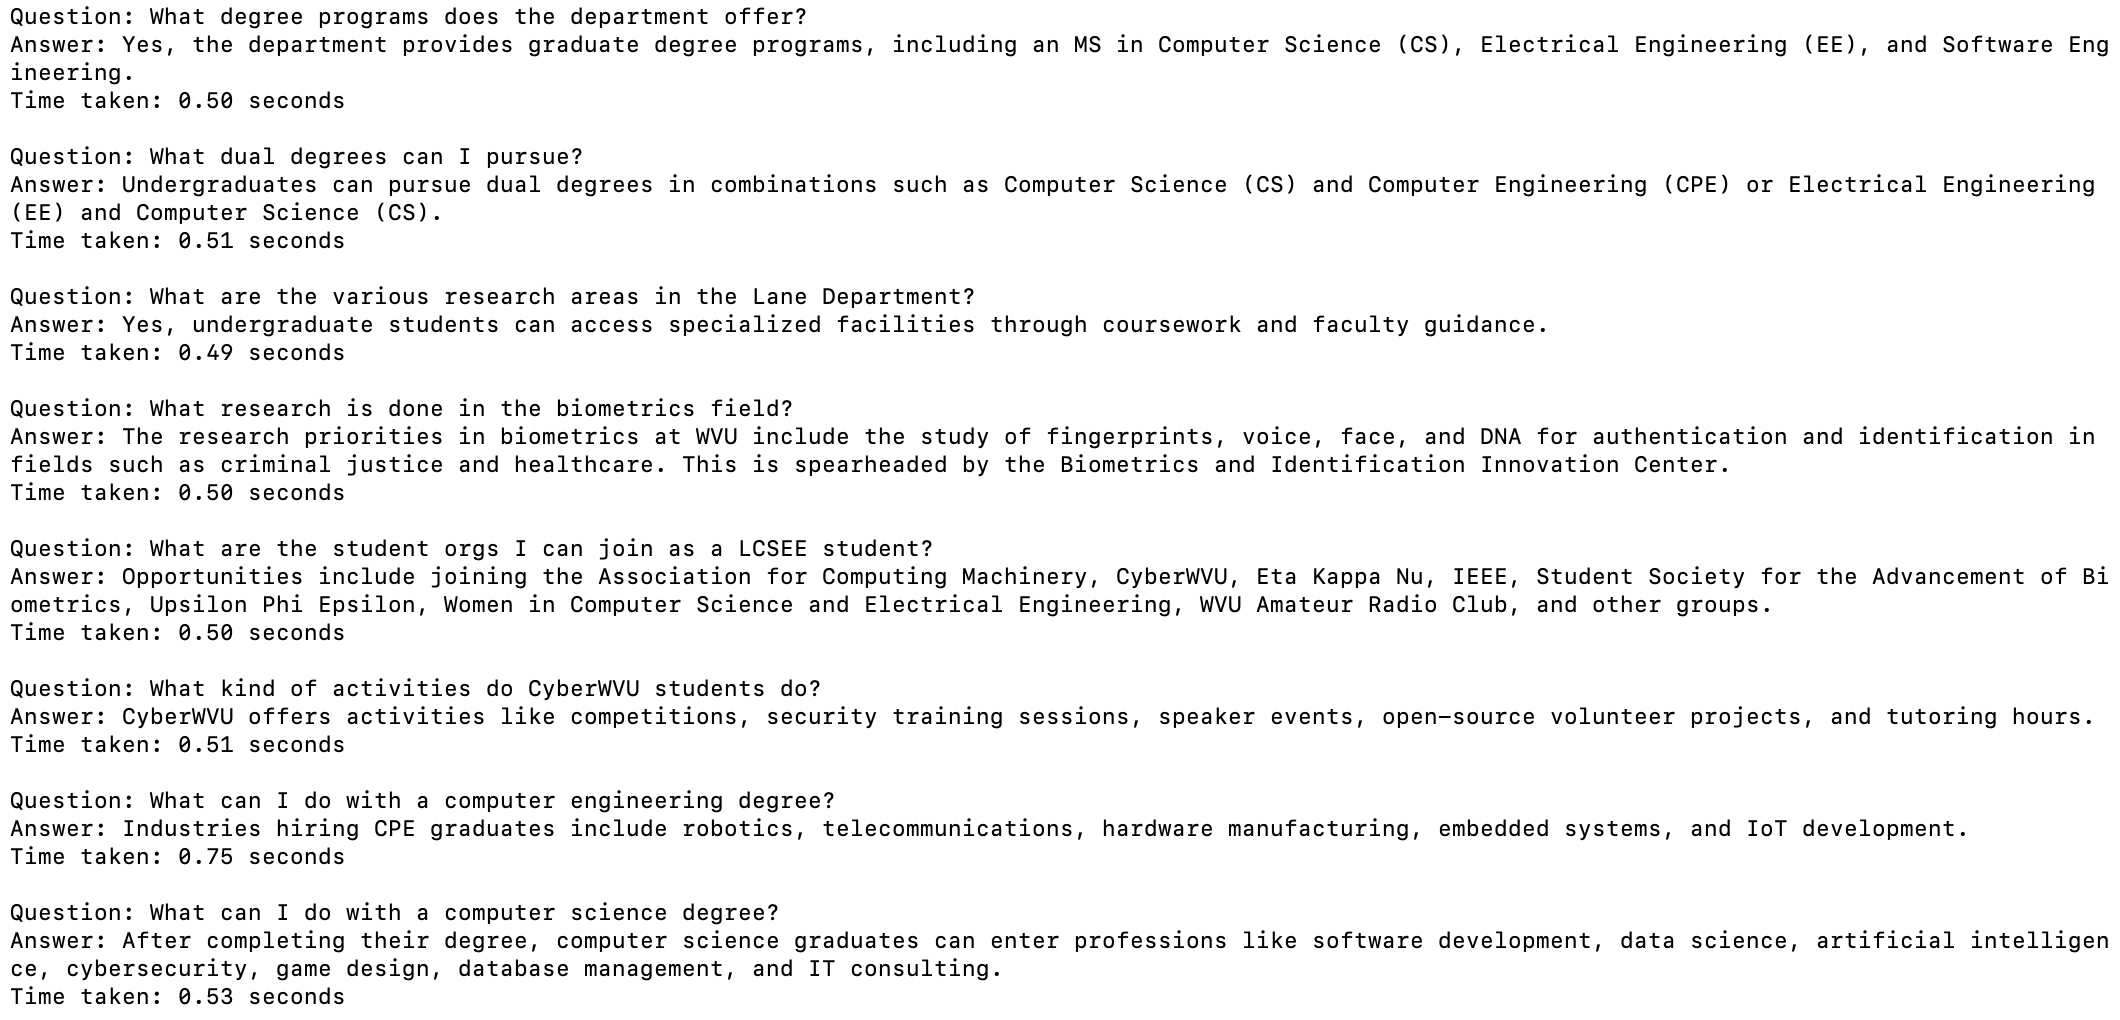
\includegraphics[width=\linewidth]{assets/CRG2_out.png}
    \caption{CRG-2 Output: SVM + NER + EKI}
    \label{fig:CRG_2-Out}
\end{figure*}

\newpage
\begin{figure*}[!h]
    \centering
    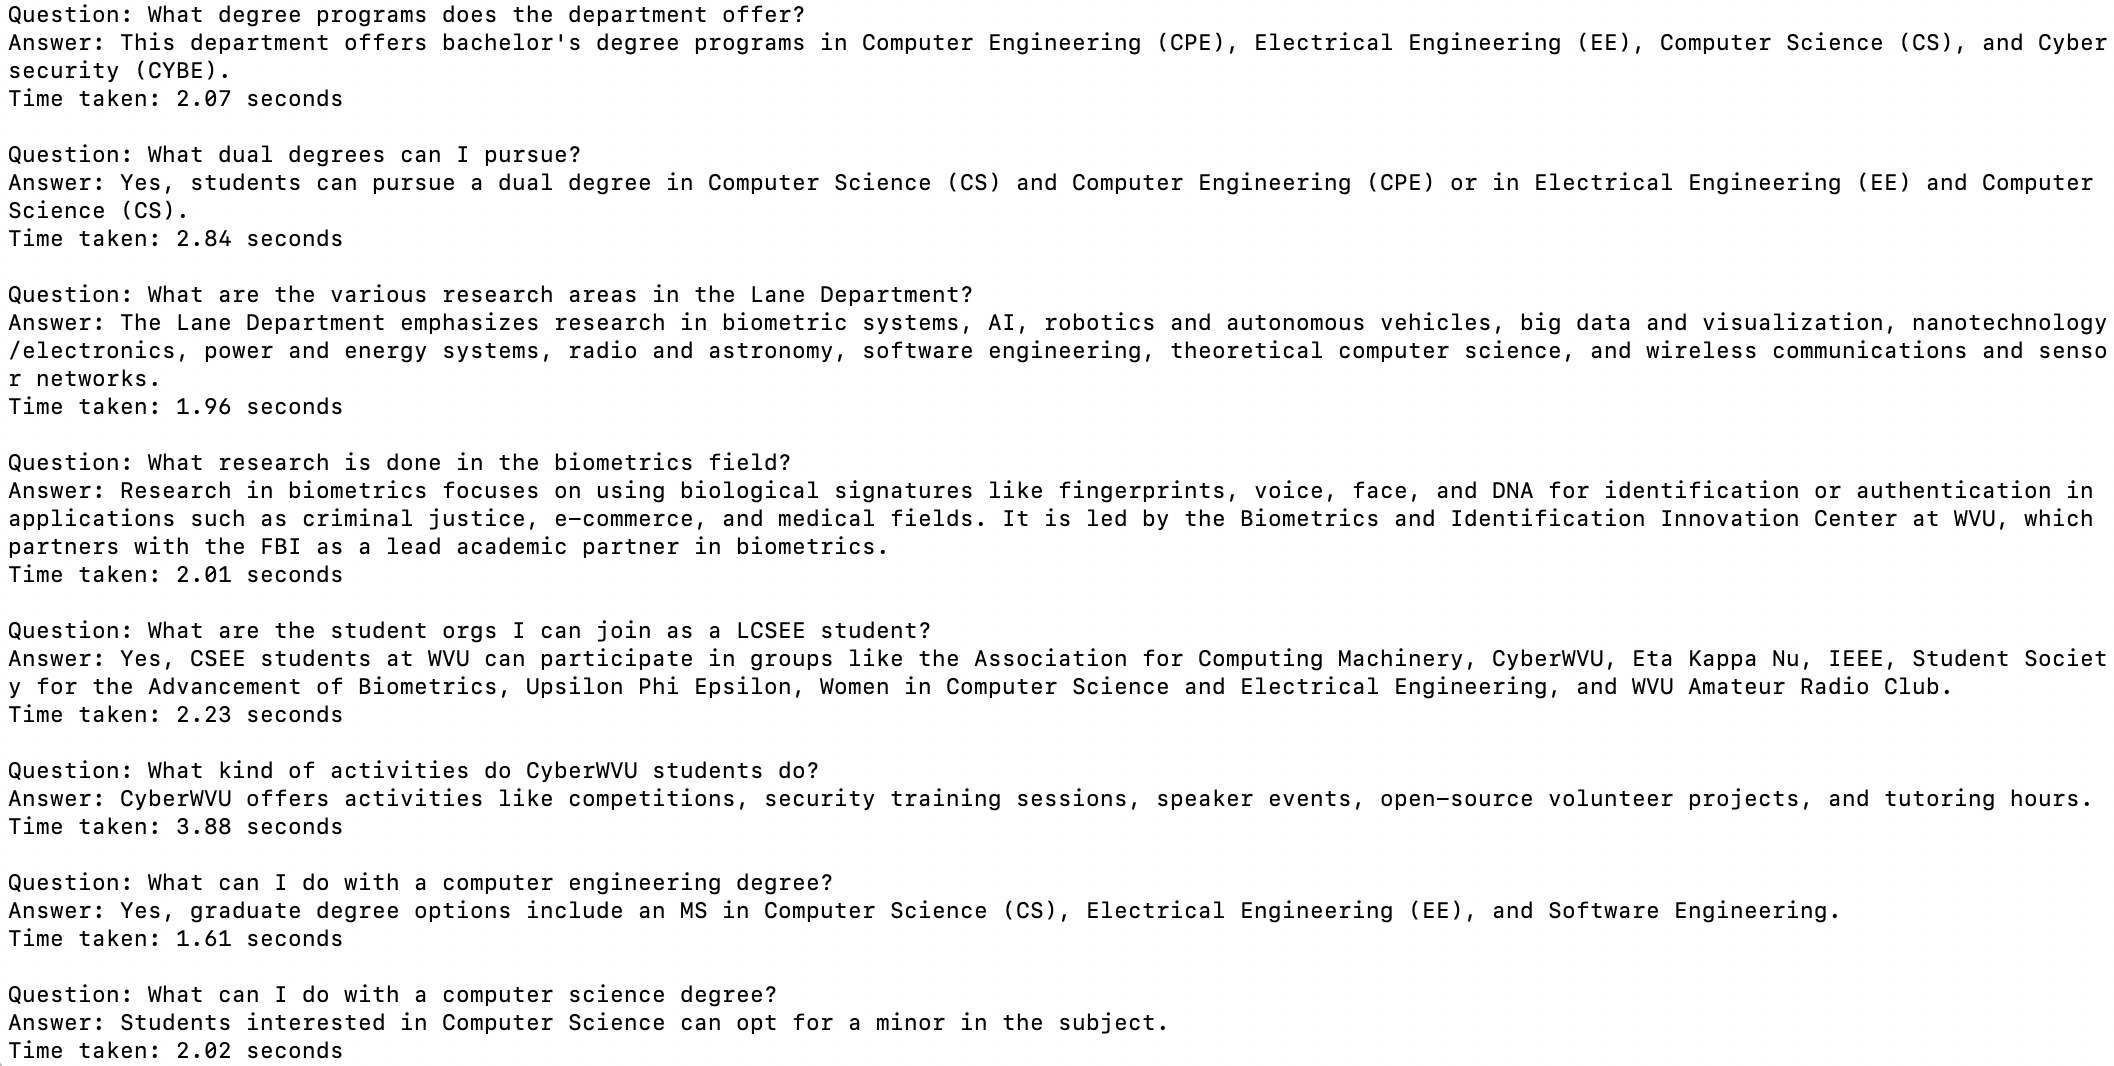
\includegraphics[width=\linewidth]{assets/CRG3_out.png}
    \caption{CRG-3 Output: DistilBERT + Vector + Cosine Similarity}
    \label{fig:CRG_3-Out}
\end{figure*}


\end{document}
